\documentclass{article}

\usepackage[utf8]{inputenc}
\usepackage{graphicx}
\graphicspath{ {Project2/figures/} }
\usepackage{float}
\usepackage{listings}
\usepackage{amsmath}
\usepackage{amssymb}
\usepackage{mathtools}
\usepackage{commath}
\usepackage{tabularx}
\usepackage[ruled,vlined]{algorithm2e}
\usepackage{caption}
% \usepackage{subcaption}
\usepackage[outputdir=../]{minted}
\usepackage{verbatim}
\usepackage{tikz}
\usetikzlibrary{arrows.meta} 
\usepackage{bm}

\usepackage{comment}
\usepackage[style=apa]{biblatex}
\addbibresource{Project3/refs.bib}

\usepackage{subfig}

\usepackage{amsthm}
\usepackage{enumitem}
\usepackage{breakcites}

\newtheorem{theorem}{Theorem}[section]
\newtheorem{lemma}[theorem]{Lemma}
\theoremstyle{definition}
\newtheorem{definition}{Definition}[subsection]

% \bibliographystyle{apalike}
\usepackage{hyperref}
\usepackage{cleveref}
\hypersetup{breaklinks=true,colorlinks=true,linkcolor=blue,citecolor=blue,filecolor=magenta,urlcolor=blue}

\DeclareMathOperator*{\argmax}{arg\,max}
\DeclareMathOperator*{\argmin}{arg\,min}
\DeclareMathOperator*{\sgn}{sgn}
\DeclareMathOperator*{\Bias}{Bias}
\DeclareMathOperator*{\Var}{Var}
\DeclareMathOperator*{\diag}{diag}

\counterwithin{figure}{section}


\title{Solving the 1-D Heat Equation using PINNs and Forward Euler}
\author{Femtehjell, Hoel and Steeneveldt}



% \def\@bibdataout@aps{%
% \immediate\write\@bibdataout{%
% @CONTROL{%
% apsrev41Control%
% \longbibliography@sw{%
%     ,author="08",editor="1",pages="1",title="0",year="1"%
%     }{%
%     ,author="08",editor="1",pages="1",title="",year="1"%
%     }%
%   }%
% }%
% \if@filesw \immediate \write \@auxout {\string \citation {apsrev41Control}}\fi
% }

\begin{document}

\setminted[python]{frame=lines,
    framesep=2mm,
    linenos,
    fontsize=\footnotesize,
    mathescape=true,
    escapeinside=||
}

\maketitle
\begin{figure}[H]
    \centering
    
\includegraphics[scale=0.5]{1797261_uio-logo.png}
\end{figure}
\newpage
\tableofcontents

\newpage
\listoffigures

\newpage

\begin{abstract}
    abstract will go here :)
\end{abstract}

\section{Intro 2: Electric Boogaloo}
Partial differential equations (PDEs) are one of the most applicable areas of mathematics. They describe how things move in relation to each other, being able to accurately describe the laws of physics which govern how fluids move, to describing the dynamics of how the stock market moves. More precisely, a PDE is an equation that describes the dynamic of a system or the relationship between a function and its derivatives.

The most interesting PDEs are usually hard to solve, and often don't even have a solution. To get around this, we use numerical algorithms to find an approximation to the solution. These algorithm can however quickly turn computationally costly for a required accuracy, and can be hard to come up with or implement.

This is where machine learning enters the picture. As machine learning has become more popular due to the increase in computational power, it has seen a vast range of applications, and solving PDEs are no exception. A key point is that regular regression methods won't get us to our goal, as we initially only have a few conditions to work from. To avoid this issue, we \textit{inform} our network of the underlying problem, such that it is able to produce results which corresponds with the rules which we have imprinted it with.

In this project, we aim to train a neural network to solve the heat equation, and see how it holds up to the analytic solution, and compare it to a simple numeric solution by the method of finite differences.

\begin{comment}
\section{Introduction}
Partial differential equations (or PDEs) are one of the most applicable areas of mathematics, ranging from fluids such as water waves, oil or aerodynamics of planes to Black-Scholes and stock prices in finance and much more. A PDE is an equation that describe the dynamic of a system or the relationship between a function and its derivatives and is dependent on multiple variables. The most interesting PDEs are usually hard to solve and sometimes don't even have a solution. To get around this, we use numerical algorithms to find an approximation to the solution. But even the numerical algorithms can sometimes be hard to come up with or implement. This leads us to machine learning. As machine learning has become more popular due to the increase in computational power, it has seen a wast range of applications and solving PDEs are no exception. \\
\newline
In this project, we aim to train a neural network to solve the one dimensional diffusion equation and compare it to both the analytical solution and a numerical solution by the method of finite differences. \\
First we will take a look at the theory, in which we will see how to solve the PDE analytically and numerically along with a brief recap of the theory of neural network (see project 2). Next, we will show how we chose to implement the theory, before we go over to discuss and show the result. Lastly we will give our final thoughts in a conclusion at the end.
\end{comment}

\newpage
\section{Theory}

\subsection{Partial differential equations}
A differential equation describes the relationship between the derivatives of an unknown function. If our unknown function is multivariate the derivatives are partial derivatives, giving a partial differential equation (PDE).
A PDE's order is the highest order derivative in the equation. A general second order PDE for the function $u(x_1, x_2, \ldots, x_n)$ looks like this
%source: https://multiphysics.us/PDE.html#:~:text=Partial%20Differential%20Equations%20(PDE)%20are,%2Cx1%2C...
\begin{equation}
    F\left( \frac{\partial^2 u}{\partial x_1 \partial x_1 }, \ldots, \frac{\partial^2 u}{\partial x_1 \partial x_n}, \ldots, \frac{\partial u}{\partial x_1}, \ldots, \frac{\partial u}{x_n}, x_1, \ldots, x_n\right)   = F(u, \mathbf{x}) = 0  \label{eq:general_pde}\\
\end{equation}

A function $u$ which satisfies this relationship is said to be a solution of the PDE. If such a solution exists it is often not unique unless further conditions are specified. In the context of a PDE where one of the variables represents time ($t$), these conditions are usually initial and boundary conditions. Initial conditions specify the value of $u(x_1 ,x_2, ..., x_n, t)$ at the initial moment 
\begin{equation*}
    u(x_1, x_2, ..., x_n, t=0) = f(x_1, ..., x_n),
\end{equation*}
where $f$ is some function.

Boundary conditions determine the behavior of the function $u$ at the boundary of a specific spatial region $D \subset \mathbb{R}^{n}$, for the $n-1$ spatial dimensions. We can denote these as
\begin{equation*}
    u(\boldsymbol{x_{\text{boundary}}}, t) = h(\boldsymbol{x_{\text{boundary}}}, t),
\end{equation*}
for some function $h$.

\subsection{The heat equation}
The heat equation is given by
\begin{equation*}
    \frac{\partial u}{ \partial t} = \alpha \left(\frac{\partial^2 u}{\partial x_1^2} + \frac{\partial^2 u}{\partial x_2^2} +... + \frac{\partial^2 u}{\partial x_n^2}\right),
\end{equation*}
where $\alpha$ is a positive constant denoting the thermal diffusivity of the material in question. The other factor of the right side is called the Laplacian of $u$ denoted $\Delta u$ or $\nabla^2 u$. Giving
\begin{equation*}
    \frac{\partial u}{\partial t} = \alpha \nabla^2 u.
\end{equation*}
If we restrict ourselves to only one spacial dimension, we get
\begin{equation*}
    \frac{\partial u}{ \partial t} = \alpha \frac{\partial^2 u}{\partial x_1^2}  .
\end{equation*}

This can be simplified by dropping the indexation of $x$ and using the notational convention $u_{xx} = \frac{\partial^2 u}{\partial^2 x} $ and $u_t = \frac{\partial u}{\partial t}$, giving the simple form
\begin{equation*}
    u_t = \alpha u_{xx}.
\end{equation*}
In this project, we will use the one dimensional heat equation, with $\alpha = 1$. The following boundary and initial conditions then apply:
\begin{align}
    u(0, t) &= 0            &\forall &t \geq 0, \nonumber \\
    u(1, t) &= 0            &\forall &t \geq 0, \label{eq:equation_conditions} \\
    u(x, 0) &= \sin(\pi x)  &\forall &x \in (0, 1). \nonumber
\end{align}

% In this project we limit ourselves to this one dimensional heat equation. With the initial condition $u(x, 0) = \sin(\pi x)$ and the boundary conditions $u(t,x) = 0 $ $\forall x \notin (0,1)$ and $\alpha = 1$

% \begin{equation}
%     \begin{cases}
%         u_{xx} = u_t & x \in (0,1), \quad t > 0 \\
%         u(0,t) = u(1,t) = 0 & t \geq 0 \\
%         u(x,0) = \sin(\pi x) & 0 < x < 1 \label{eq:equation_conditions}
%     \end{cases}
% \end{equation}


\subsubsection{Physical interpretation}
There are many ways to interpret the heat equation physically, but by far the easiest and most used example is the heat in a rod. Thus we have a rod of length $1$. $u$ is thus a surface and $u(t,x)$ denotes the temperature at time $t$ and position $x$ on the rod. As our boundary conditions are $u(0,t) = u(1,t) = 0$, the temperature at the ends of the rod is always zero. At time $t = 0$, the temperature of the rod is given by
\begin{equation*}
    u(x,0) = \sin(\pi x).
\end{equation*}
This temperature is at its maximum at the middle of the rod, $x=\tfrac{1}{2}$. The function $u$ thus describes how this initial peak temperature at the rod's center diffuses along the rod over time.

\subsubsection{Analytical solution}
To analytically solve this equation, we use separation of variables. We need to find a family of particular solutions $\{u_k(x,t)\}$. $u(x,t)$ would then be a sum of different solutions by the principle of superposition. This sum would then be
\begin{equation*}
    u(x,t) = \sum_{k}c_ku_k(x,t) \qquad k = 0,1,2,\dots
\end{equation*}
where $c_k$ is the Fourier coefficient. This means that our initial condition can be written as
\begin{equation*}
    f(x) = \sum_{k}c_ku(x,0) = \sum_k c_k\sin(\pi x) = \sin(\pi x)
\end{equation*}
hence, $c_k = 1$ for some $k$ and zero for all other values of $k$. This means we can omit the full derivation of the general method for separation of variables using Fourier coefficients. 
We start by assuming that the solution has the form
\begin{equation*}
    u(x,t) = X(x)T(t).
\end{equation*}
In the context of our equation, we get
\begin{gather*}
    X(x) T'(t) = X''(x) T(t) \\
    \frac{X''(x)}{X(x)} = \frac{T'(t)}{T(t)}. 
\end{gather*}

Since the left side is a function of $x$ alone and the right side is a function of $t$ alone, they must both equal a constant value, which we denote as $-\lambda$. The negative coefficient is chosen for convenience. This leads us to form the two separate ordinary differential equations (ODEs)
\begin{equation*}
    X''(x) + \lambda X(x) = 0,\quad \text{and} \quad T'(t) + \lambda T(t) = 0. 
\end{equation*}
Solving these ODEs will give us functions $X(x)$ and $T(t)$ that compose the solution $u(x,t)$.

For $T$ we get the simple solution
\begin{equation*}
    T(t) = E e^{-\lambda t},
\end{equation*}
while for $X$ we get two complex roots, hence the solution 
\begin{equation*}
    X(x) = C \cos\left(\sqrt{\lambda}x\right) + D \sin\left( \sqrt{\lambda}x \right).
\end{equation*}
Using the boundary conditions, we know that $u(0, t) = 0$, so
\begin{equation*}
    X(0) = 0 = C \cos\left(\sqrt{\lambda} \cdot 0\right) + D \sin\left( \sqrt{\lambda} \cdot 0 \right) = C.
\end{equation*}
Thus $C = 0$. As we assumed the solution to the PDE was $X(x) T(t)$, we get
\begin{equation*}
    u(x, t) = X(x) T(t) = E e^{-\lambda t} D \sin\left( \sqrt{\lambda} x \right).
\end{equation*}
Using the initial value $u(x, 0) = \sin(\pi x)$ we get
\begin{equation*}
    \sin(\pi x) = E e^{-\lambda \cdot 0} D\sin\left( \sqrt{\lambda}x \right) = ED \sin\left( \sqrt{\lambda}x \right).
\end{equation*}
Hence, $\lambda = \pi^2$, and $ED = 1$. Our final expression for the differential equation is thus
\begin{equation}
    u(x, t) = e^{-\pi^2 t} \sin(\pi x).
    \label{eq:analytical_sol}
\end{equation}

In order to verify that our solution is correct, we first differentiate with respect to $t$, giving
\begin{equation*}
    u_t = -\pi^2 e^{-\pi^2 t} \sin(\pi x).
\end{equation*}
Differentiating with respect to $x$ gives
\begin{align*}
    u_x &= \pi e^{-\pi^2 t} \cos(\pi x) \\
    u_{xx} &= -\pi^2 e^{-\pi^2 t} \sin(\pi x),
\end{align*}
indeed verifying that $u_{t} = u_{xx}$, meaning we have our analytical solution.

\begin{comment}
\subsubsection{Analytical solution}
To solve this equation analytically, we will use the method of separation of variables. Assume that the solution to the equation is of the form
\begin{equation*}
    u(x,t) = X(x)T(t)
\end{equation*}
inserting it into our equation, we get
\begin{equation*}
    X''(x)T(t) = X(x)T'(t)
\end{equation*}
dividing both sides with the assumed solution
\begin{equation*}
    \frac{X''(x)}{X(x)} = \frac{T'(t)}{T(t)}
\end{equation*}
Since both sides of the equation only depends on its own variable, they must equal a constant
\begin{equation*}
    \frac{X''(x)}{X(x)} = \frac{T'(t)}{T(t)} = -\lambda,
\end{equation*}
where the minus sign is used for convenience. Now we have the two ordinary differential equations
\begin{equation*}
    \begin{split}
        X''(x) + \lambda X(x) & = 0 \\
        T'(t) + \lambda T(t) & = 0
    \end{split}
\end{equation*}
For $T$, we have a simple solution
\begin{equation*}
    T(t) = Ee^{-\lambda t}
\end{equation*}
For $X$, we see that we get two complex roots, hence the solution to the differential equation is
\begin{equation*}
    X(x) = Ccos(\sqrt{\lambda}x) + D\sin(\sqrt{\lambda}x)
\end{equation*}
and by using the boundary conditions, we know that $u(0,t) = 0$ and thus
\begin{equation*}
    \begin{split}
        X(0) & = 0 \\
        & = Ccos(\sqrt{\lambda} 0) + D\sin(\sqrt{\lambda} 0) \\
        & = C
    \end{split}
\end{equation*}
hence, $C = 0$. Since we assumed the solution to the PDE was $X(x)T(t)$, we get
\begin{equation*}
    u(x,t) = X(x)T(t) = Ee^{-\lambda t}D\sin(\sqrt{\lambda}x)
\end{equation*}
Using the initial value, we see that
\begin{equation*}
    \begin{split}
        u(x,0) & = \sin(\pi x) \\
        & = Ee^{-\lambda 0}D\sin(\sqrt{\lambda}x)
    \end{split}
\end{equation*}
hence, $\lambda = \pi^2$ and either $E = D = 1$ or $ED = 1$ and so our final expression for the differential equation is
\begin{equation*}
    u(x,t) = e^{-\pi^2t}\sin(\pi x)
\end{equation*}
Checking to see if this is correct, we first differentiate w.r.t $t$
\begin{equation*}
    u_t = -\pi^2e^{-\pi^2t}\sin(\pi x)
\end{equation*}
and differentiating w.r.t $x$
\begin{equation*}
    \begin{split}
        u_x & = \pi e^{-\pi^2t}cos(\pi x) \\
        u_{xx} & = -\pi^2e^{-\pi^2t}\sin(\pi x)
    \end{split}
\end{equation*}
hence, we see that
\begin{equation*}
    u_{xx}(x,t) = u_t(x,t)
\end{equation*}
and we have an analytical solution to the equation.
\end{comment}

\subsection{Finite differences}
\subsubsection{Approximation of the derivative}
Recall that the definition of the derivative is given by
\begin{equation*}
    f'(x) = \lim_{h \to 0} \frac{f(x + h) - f(x)}{h}.
\end{equation*}
Working numerically, this expression has to be approximated. This leads to the forward difference approximation
\begin{equation*}
    f'(x) \approx \frac{f(x + h) - f(x)}{h},
\end{equation*}
and the backward difference approximation
\begin{equation*}
    f'(x) \approx \frac{f(x) - f(x - h)}{h}.
\end{equation*}
Note that in the approximation $h$ is a fixed (small) number called the step size, as we cannot take the limit numerically. Combining these, we get the centered difference
\begin{gather*}
    2f'(x) \approx \frac{f(x + h) - f(x)}{h} + \frac{f(x) - f(x - h)}{h} = \frac{f(x + h) - f(x - h)}{h} \\
    f'(x) \approx \frac{f(x + h) - f(x - h)}{2h}.
\end{gather*}

Extending this to the second derivative, we find
\begin{gather*}
    f''(x) \approx \frac{f'(x + h) - f'(x)}{h} \approx \frac{\left( f(x + h) - f(x) \right) - \left( f(x) - f(x - h) \right)}{h^2} \\
    f''(x) \approx \frac{f(x + h) - 2f(x) + f(x - h)}{h^2},
\end{gather*}
where we applied the backward differences.

Applying this in the context of our function $u$ with a stepsize $\Delta t$ in $t$-direction and $\Delta x$ in $x$-direction, we get
\begin{gather*}
    u_t \approx \frac{u(x, t + \Delta t) - u(x,t)}{\Delta t} \\
    u_{xx} \approx \frac{u(x + \Delta x, t) - 2u(x, t) + u(x - \Delta x, t)}{\Delta x^2}.
\end{gather*}
Based on our stepsizes, we define our grid points by $x_i = i \Delta x, t_j = j\Delta t$, and write $u_{i,j} = u(x_i, t_j)$. Note that $t_{j+1} = (j + 1)\Delta t = t_j + \Delta t$. We can now simplify our notation for the approximations into
\begin{gather*}
    u_t \approx \frac{u_{i, j+1} - u_{i,j}}{\Delta t}, \\
    u_{xx} \approx \frac{u_{i+1,j} - 2u_{i,j} + u_{i-1,j}}{\Delta x^2}.
\end{gather*}

\subsubsection{Explicit forward Euler}
Our original equation $u_t = u_{xx}$ can now be written in the discretized form
\begin{align*}
    \frac{u_{i, j+1} - u_{i,j}}{\Delta t} &= \frac{u_{i+1,j} - 2u_{i,j} + u_{i-1,j}}{\Delta x^2} \\
    u_{i, j+1} - u_{i,j} &= \frac{\Delta t}{\Delta x^2} \left( u_{i+1,j} - 2u_{i,j} + u_{i-1,j} \right) \\
    u_{i, j+1} &= u_{i,j} + \frac{\Delta t}{\Delta x^2} \left( u_{i+1,j} - 2u_{i,j} + u_{i-1,j} \right).
\end{align*}
Writing $\alpha = \frac{\Delta t}{\Delta x^2}$, we get the explicit scheme
\begin{align*}
    u_{i, j+1} &= u_{i,j} + \alpha \left( u_{i+1,j} - 2u_{i,j} + u_{i-1,j} \right) \tag{\theequation}\label{eq:forwardEuler}\\
    &= u_{i,j} + \alpha u_{i+1,j} - 2\alpha u_{i,j} + \alpha u_{i-1,j} \\
    &= \alpha u_{i+1,j} + (1 - 2\alpha) u_{i,j} + \alpha u_{i-1, j}.
\end{align*}

Note that as the iteration is only dependent on previous time steps, the scheme is explicit. With $x \in [0, L]$ and $n+2$ points, we get a step size $\Delta x = \frac{L}{n+1}$. $x_0, x_{n+1}$ are then our boundary points, such that $u_{0, j} = 0 = u_{n+1, j}$ constant. With this we write our points at time step $j$ as the vector
\begin{equation*}
    V_j = [u_{1, j}, \ u_{2, j} \ , \ldots \ , u_{n, j}]^T,
\end{equation*}
with $u_{i,0} = \sin(\pi x_i)$.

With the tridiagonal $n \times n$ matrix $A$ defined by
\begin{equation*}
    A = 
    \begin{bmatrix}
        1 - 2\alpha & \alpha & & & \\
        \alpha & 1 - 2\alpha & \alpha & & \\
        & \alpha & 1 - 2\alpha & & \\
        & & \ddots & \ddots & \\
        & & & \alpha & 1 - 2 \alpha
    \end{bmatrix},
\end{equation*}
where we use the convention of leaving zeros blank, we can express our explicit scheme by
\begin{equation} \label{eq:MatrixVecExpr}
    u_{i,j}
    =
    \begin{cases}
        0           & \text{for } i = 0, \\
        (A V_j)_i   & \text{for } 1 \leq i \leq n, \\
        0           & \text{for } i = n + 1.
    \end{cases}
\end{equation}
Alternatively, we have $V_{j+1} = AV_j$. The scheme defined by (\ref{eq:forwardEuler}) is known as the Explicit Forward Euler scheme. Note that as $V_{j+1} = AV_j$, we can explicitly calculate a time step $k$ by $V_k = A^k V_0$.

A tridiagonal Toeplitz $n \times n$ matrix is of the form
\begin{equation*}
    T = \begin{bmatrix}
        b & c &  &  & \\
        a & b & c &  & \\
         & a & b &  & \\
         &  & \ddots & \ddots & \\
         &  &  & a & b \\
    \end{bmatrix},
\end{equation*}
denoted $T = (n; a, b, c)$, and is known to have eigenvalues $\lambda_h = b + 2\sqrt{ac} \cos(\frac{h\pi}{n + 1})$ for $h = 1, 2, \ldots, n$ \parencite{toeplitz}. Note that in our case $A$ is tridiagonal, Toeplitz and symmetric of the form $A = (n; \alpha, 1 - 2\alpha, \alpha)$, meaning it's eigenvalues are
\begin{equation*}
    \lambda_h = (1 - 2\alpha) + 2\alpha \cos\frac{h\pi}{n + 1} \qquad \text{for } h = 1, 2, \ldots, n.
\end{equation*}

In order for our method to reach a definite value after a finite number of time steps, we require that the spectral radius $\rho(A) < 1$ \parencite[p.~511]{matrixcomp}. Treating the eigenvalues as functions of $h$, we find by differentiation, that
\begin{equation*}
    \frac{\partial \lambda_h}{\partial h} = -\frac{2\alpha\pi}{n+1}\sin\frac{h\pi}{n+1},
\end{equation*}
which is strictly decreasing for $h \in [1, n]$. Thus our largest eigenvalue in absolute value is either $\lambda_1$ or $\lambda_n$. In the first case we find
\begin{equation*}
    \lambda_1 = (1 - 2\alpha) + 2\alpha \cos\frac{1\pi}{n + 1} < 1 - 2 \alpha + 2\alpha = 1.
\end{equation*}

In the other end we find
\begin{equation*}
    \lambda_n = (1 - 2\alpha) + 2\alpha \cos\frac{n\pi}{n + 1} > 1 - 2\alpha - 2\alpha = 1 - 4\alpha,
\end{equation*}
meaning that for the spectral requirement to be satisfied we must have
\begin{align*}
    1 - 4\alpha &> -1 \\
    4 \alpha &< 2 \\
    \alpha &< \frac{1}{2}.
\end{align*}
Thus, when implementing the scheme, we require that $\alpha=\frac{\Delta t}{\Delta x^2} < \frac{1}{2}$.

This reveals a major drawback of this method, as with just 1 000 steps in $x$, we require 2 000 000 steps in $t$, growing quadratically as we increase the number of $x$ steps.

\subsection{Neural networks}
A neural network is composed of interconnected nodes arranged in layers. The initial layer is the input layer, the final layer is the output layer, and the intervening layers—called hidden layers—are responsible for processing the inputs into the final output. 

In this project we wish to find an approximation of the function $u$ which satisfies the conditions given by \eqref{eq:equation_conditions}. Our network will thus have two input nodes ($t$ and $x$) and a single output node $u$, the temperature. We'll also be limiting ourselves to fully connected neural networks, that is each node is connected to every node in the next layer. Thus obtaining a model depicted by \autoref{fig:FullyConnectedFeedForward}.

\begin{figure}[ht]
\centering
\def\layersep{3cm}
\def\nodeinlayersep{2cm}
\begin{tikzpicture}[>=Stealth,
    % Define the style for each layer
    neuron/.style={circle, fill=black!25, minimum size=12pt, inner sep=0pt},
    input neuron/.style={neuron, fill=red!50},
    output neuron/.style={neuron, fill=orange!50},
    hidden neuron/.style={neuron, fill=blue!50},
    % Define the style for the connecting lines
    connection/.style={->,shorten <=1pt}
]

% Determine the separation between neurons and layers
\def\nodeinlayersep{1cm}  % Separation between nodes in the same layer
\def\layersep{2.5cm}      % Separation between layers

% Define the first hidden layer with 6 neurons using a loop
\foreach \name / \y in {1,...,6}
    \node[hidden neuron] (H1-\name) at (\layersep,-\y * \nodeinlayersep + 2.5*\nodeinlayersep) {};
\node (H1-vdots-top) at (1*\layersep, 0.9*\layersep) {$\vdots$};
\node (H1-vdots-bottom) at (1*\layersep, {-6.8 * \nodeinlayersep + 2.5*\nodeinlayersep}) {$\vdots$};

% Define the last hidden layer, also with 6 neurons
\foreach \name / \y in {1,...,6}
    \node[hidden neuron] (H2-\name) at (3*\layersep,-\y * \nodeinlayersep + 2.5*\nodeinlayersep) {};
\node (H2-vdots-top) at (3*\layersep, 0.9*\layersep) {$\vdots$};
\node (H2-vdots-bottom) at (3*\layersep, {-6.8 * \nodeinlayersep + 2.5*\nodeinlayersep}) {$\vdots$};

% Input layer with ellipsis to imply an arbitrary number of neurons
\node[input neuron] (I-1) at (0,-2.5*\nodeinlayersep + 2.5*\nodeinlayersep) {};
\node[input neuron] (I-2) at (0,-4*\nodeinlayersep + 2.5*\nodeinlayersep) {};


% Output layer neuron
\node[output neuron] (O) at (4*\layersep,-3*\nodeinlayersep + 2.5*\nodeinlayersep) {};

% Connect the input layer to the first hidden layer
\foreach \source in{1,2}
    \foreach \dest in {1,...,6}
        \draw [connection](I-\source) -- (H1-\dest);
    

% Connect the last hidden layer to the output layer
\foreach \source in {1,...,6}
    \draw [connection] (H2-\source) -- (O);

% HERE: repeat such that there are 6 horizontal dots in the middle of picture
\node (H-dots-1) at (2*\layersep,-2*\nodeinlayersep + 2.5*\nodeinlayersep) {$\dots$};
\node (H-dots-2) at (2*\layersep,-3*\nodeinlayersep + 2.5*\nodeinlayersep) {$\dots$};
\node (H-dots-3) at (2*\layersep,-4*\nodeinlayersep + 2.5*\nodeinlayersep) {$\dots$};
\node (H-dots-4) at (2*\layersep,-5*\nodeinlayersep + 2.5*\nodeinlayersep) {$\dots$};

\end{tikzpicture}
\caption{Illustration of a feed-forward pass in a fully connected neural network with two inputs (red), an arbitrary number of hidden layers, each with arbitrary nodes (blue), and one output node (orange).}
\label{fig:FullyConnectedFeedForward}
\end{figure}
\begin{comment}
\subsubsection{Regression}

In a naive regression framework, a neural network treats the problem of approximating the function $u$ purely as a data-driven exercise, mapping inputs $(t, x)$ to output $u$ without explicit regard to the physical principles that define the system, encapsulated in equation \eqref{eq:equation_conditions}. Such an approach might inadvertently ignore crucial aspects of the system's behavior and fail to generalize to conditions not represented in the training set.

The cost function for such a setup might look like this
\begin{equation*}
    C(\theta) = \underbrace{\frac{1}{N} \sum_{i=1}^{N} \left( u_{\text{predicted}}^{(i)}(\theta) - u_{\text{true}}^{(i)} \right)^2}_{\text{MSE Term}} + \underbrace{ \lambda || W||_L}_{\text{Regularization Term}}.
\end{equation*}
Here, $u_{\text{predicted}}^{(i)}$ represents the neural network's output for the $i$-th input sample, $u_{\text{true}}^{(i)}$ denotes the corresponding true or observed value of $u$, $\theta$ represents the network parameters (weights and biases) and W the weights. The first term enforces the accuracy of the regression, while the second term aims to mitigate overfitting.

\end{comment}

\subsubsection{Physics-informed neural networks}

Physics-Informed Neural Networks (PINNs) offer a different framework compared to naive regression models. In a typical regression setup, the problem of approximating the function $u$ is treated as an entirely data-driven exercise. The network learns to map inputs $(t, x)$ to the output $u$, without regard of the physical laws that govern the output, as articulated by equation \eqref{eq:equation_conditions}. Such a method may neglect vital system behaviors, leading to poor generalization outside the scope of the training data.

While the traditional regression approach represents a starting point, another approach is to incorporate the physical principles governing our function $u$ directly into the model. This is achieved with Physics-Informed Neural Networks (PINNs).

For this, we define a trial solution $g$ for our problem. Which is to adhere to (\ref{eq:equation_conditions}). In general, it is of the form
\begin{equation*}
    g(x, t) = h_1(x, t) + h_2(x, t, \mathcal{N}(x, t, \theta)).
\end{equation*}
Here, $\mathcal{N}$ represents our neural network with the weights and biases from $\theta$. In addition, $h_1$ should by itself make sure that our solution satisfies the given conditions.

We can satisfy the initial conditions for our 1d heat equation with
\begin{equation*}
    g(x, t) = (1 - t) \sin(\pi x) + t \cdot \mathcal{N}(x, t, \theta),
\end{equation*}
and noting that $\sin(0) = \sin(\pi) = 0$, we can satisfy the boundary requirements simply with
\begin{equation*}
    g(x, t, \theta) = (1 - t) \sin(\pi x) + tx (1 - x) \cdot \mathcal{N}(x, t, \theta).
\end{equation*}

As we are attempting to solve for a solution which satisfies $u_t = u_{xx}$, we can express this as minimizing $\left(u_t - u_{xx}\right)^2$, or rather our approximation
\begin{equation*}
    \left( \frac{\partial g}{\partial t} - \frac{\partial^2 g}{\partial x^2} \right)^2.
\end{equation*}
This then becomes the basis for our loss function $L(x, t; \theta)$. As discussed in greater detail in our previous project, we approximate the derivatives through automatic differentiation.

For a given set of values $\left\{ (x_i, t_i) \right\}_{i=0}^{N}$, our cost function thus becomes
\begin{equation*}
    C(\boldsymbol{x}, \boldsymbol{t}, \theta) = \frac{1}{N + 1} \sum_{i=0}^N \left( \frac{\partial g}{\partial t}(x_i, t_i) - \frac{\partial^2 g}{\partial x^2}(x_i, t_i) \right)^2.
\end{equation*}

Calculating the gradient relative to the weights of the given expression is difficult as it implicates the entire network and not solely the output layer. This means we cant use back propagation. However, the needed derivatives can be determined utilizing automatic differentiation, a method which we have elaborated on in the previous project.

This setup requires no data for interior of the domain, it simply requires sampling pairs $(x_i, t_i)$

%We then adjust our weights by $\theta_\text{new} = \theta - \lambda \nabla_\theta C(\boldsymbol{x}, \boldsymbol{t}, \theta)$, for a chosen learning rate $\lambda$, by taking the gradient with respect to $\theta$. As our expression now involves the entire neural network rather than just the output layer back propagation is no longer an option. Luckily, the derivatives can still be found through automatic differentiation, as discussed in greater detail in the previous project. It is then important to choose values $(x_i, t_i)$ such that we test for our given conditions.

\subsubsection{Activation functions and Universal Approximation theorem}
The activation functions serve as a way to introduce non-linearity into neural networks. Without them, the network becomes a linear operator, greatly reducing its ability to learn.  Which  activation function you chose is also important for model convergence and performance.

The Universal Approximation theorem states that any continuous function on a compact subset of $\mathbb{R}^{n}$ can be approximated arbitrarily well by a shallow neural network of arbitrary width. This was first proved for sigmoidal activation functions in  \textcite{universalapprox} and further extended to hold for activation functions if and only if they where non-polynomial by \textcite{pinkus_1999}. 

Many other similar and interesting results have been shown for deep (more than one layer) neural networks. Specifically \textcite{kidger2020universal} showed that for  deep narrow networks the restrictions are continuity, non affiance (not a multivariate polynomial of degree less than 2) and continuously differentiable on at least one point which is different from zero. Reflecting the greater complexity of the deep networks

However, knowing these approximates exist does not necessarily tell us how to construct them or that they will perform efficiently in practice.

The sigmoid function, also known as the logistic function, is one of the earliest activation functions used in neural networks. It maps any input to a value between 0 and 1, which is particularly useful for models where we need to predict probabilities as outputs. The shape of its curve resembles an "S," providing a smooth gradient.  However, it is susceptible to the vanishing gradient problem as the gradient approaches zero for very large or vary small especially in deep networks


\newpage
\section{Method}
\subsection{Forward Euler}
Solving numerically can quickly become computationally costly, due to the stability criterion $\frac{\Delta t}{\Delta x^2} \leq \frac{1}{2}$. As stated previously, this requires that the number of time steps grows quadratically based on the desired accuracy in the spatial dimension. Thus choosing to store all iterations quickly turns into a memory bound problem, rather than a computationally bound one.

With a desired $\Delta x = 1 / 1000$, we require at least 2 million time steps for the scheme to be stable. If we naively stored the computation for each time step, we would have to allocate space for 2 billion floating point numbers. With single precision floating point numbers, each 32bits in size, this would require us to allocate 8 gigabytes, which is practically impossible on a laptop with limited memory. Read and write operations on an array of this size quickly becomes more expensive than the computation itself.

Noticing however that the computation at one time step is only dependent on the previous one, we only require 16 kilobytes, which is hardly an issue on modern computers. Computing the iterations is however an issue in and of itself. The naive approach in this case is to just apply the expression found in (\ref{eq:MatrixVecExpr}).

Taking again the example with $\Delta x = 1 / 1000$, we would have to allocate a $1000 \times 1000$ matrix, with mostly zero elements. Computing a single time step would then require 1 million floating point operations, most of which are just zero. With the 2 million time steps required, we would have to compute 2 trillion operations. Implementing it as a sparse matrix can alleviate some of these issues, however knowing it is Toeplitz, we can still do better.

We can instead implement the iteration through vectorized operations. In this case, the iteration is more closely implemented as (\ref{eq:forwardEuler}). This has the advantage of being able to utilize SIMD (Single instruction, multiple data) instructions, where the operation is performed simultaneously across multiple values.

Still, implementing this in python can be rather slow. Even when utilizing \verb|NumPy| for the computations for an iteration, looping over the given number of iterations is slow. Due do this, we heavily utilize the library \verb|JAX| \parencite{jax2018github}. As well as being performant in the computations, it allows for just-in-time compilation, where a function is analyzed and optimized on its first call, using the optimized version for later calls. It can however be prickly with loops, requiring the number of iterations to be known at compile time. This is due to it unrolling the loop into an explicit list of instructions, which can cause the compilation itself to become slow. As we might not know the number of iterations beforehand, we use the function \verb|jax.lax.fori_loop|, which creates highly optimized loops.


%As a result, we achieved good performance, even in Python. Instead of storing the entire solution for all time points, we instead opted for storing slices along the time axis on the magnitude of 100-1000. A stark difference in the case of $\Delta x = 1/1000$ with its required 2 million time steps. This approach reduced our memory requirements without any significant loss in information for analysis purposes.

With this, we achieved good performance, even in python. A major disadvantage of this implementation however, is that we do not save the time steps as we iterate, limiting our ability to analyze how the iteration evolved over time, only being left with the final results. We can however choose to manually save a few time steps, but this has to be decided before the computation is performed.

\subsection{Neural network}
We utilized \verb|jax.grad|, \verb|jax.jacobian| and \verb|jax.hessian| in order to differentiate the functions in our PINN implementation. They all rely on automatic differentiation, however they serve slightly different goals. While \verb|grad| computes the derivative with respect to a single input, \verb|jacobian| and \verb|hessian| are able to compute partial derivatives.

With this, we are able to find all the derivatives necessary for our cost function and back propagation. Through vectorization, and the techniques mentioned previously, we were able to again achieve good performance. As this project was a lot more focused on one problem, we choose a more functional approach for our implementations, as \verb|JAX| works poorly with classes.

A major advantage of this approach, is that we are not restricted by the previous stability criterion, meaning we aren't forced to choose as many points.



\begin{comment}
    1. Aktiveringsfunksjoner
    2. Dybde / Høyde
    3. Måten vi valgte punkter
    4. Noe mer?
\end{comment}

\newpage

\section{Results}

\subsection{The Analytical Solution}
As a reference for the results here is the analytical solution of the one-dimensional Heat equation, given by
\[
u(t,x) = e^{-\pi^2 t}sin(\pi x)
\]

\begin{figure}[H]%
    \centering
    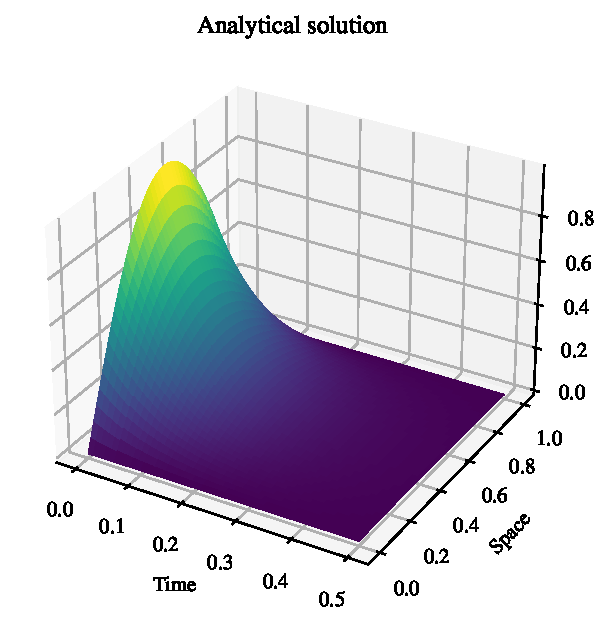
\includegraphics[width=10cm]{Project3/figures/1dHeat/Analytical_sol.pdf}
    \caption{Analytical solution of the one-dimensional Heat equation }
    \label{fig:Analytic}
\end{figure}


\subsection{Forward Euler}
For the majority of this rapport we found it most descriptive to plot the difference between the analytical approximations and our numerical solutions. For forward Euler we found that the analytical solution was greater than the numerical one. Thus the figures below are simply $u_{\text{analytical}} - u_{\text{numerical}}$
\begin{figure}[H]%
    \centering
    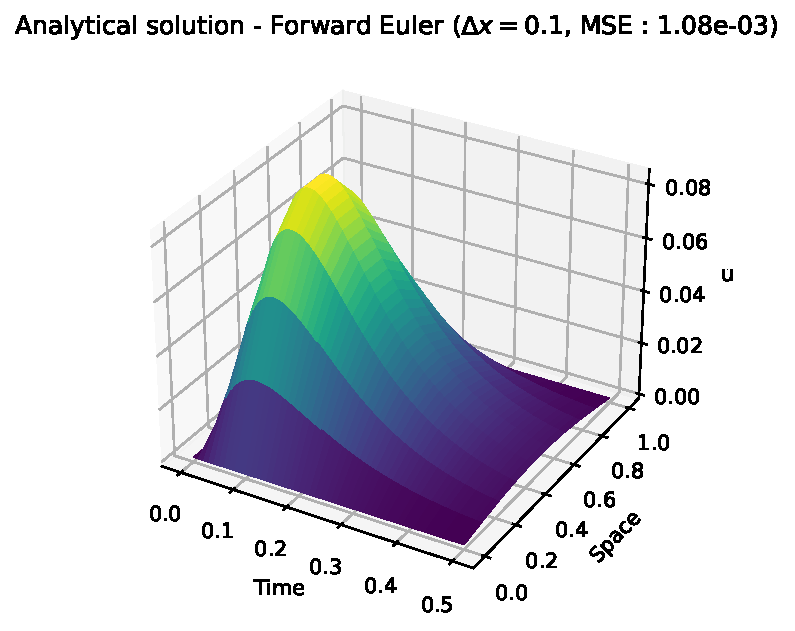
\includegraphics[width=10cm]{Project3/figures/1dHeat/dx=0.1.pdf}
    \caption{Difference between the analytical and Forward Euler solution $\Delta x = \frac{1}{10}$, $\Delta t = \frac{\Delta x^2}{2} = \frac{1}{200} $}
    \label{fig:ForwardEulerdx=0.1}
\end{figure}


\begin{figure}[H]%
    \centering
    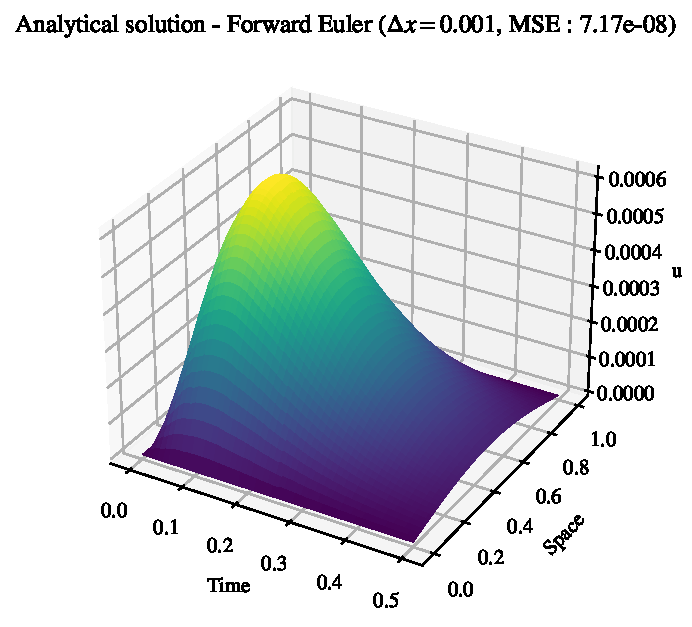
\includegraphics[width=11cm]{Project3/figures/1dHeat/dx=0.001.pdf}
    \caption{Difference between the analytical and Forward Euler solution $\Delta x = \frac{1}{1000}$, $\Delta t = \frac{\Delta x^2}{2} = \frac{1}{2000000} $}
    \label{fig:ForwardEulerdx=0.001}
\end{figure}




\subsection{Neural Networks}


\section{Discussion}
While the numerical approach was able to generate more precise results, it was highly restricted in what information we were able to extract from the problem. Per the stability criterion, a 10x increase in the spatial resolution required a 1000x increase in the total computation. The network on the other hand, was able to generalize well from a limited subset of points. Representing a higher upfront cost, once the network was trained it allowed values to be generated from arbitrary time steps, without the need for previous ones to be computed beforehand.

The approaches differed in the type of work which was required in order to get working results. While the numerical approach required a bit of pen and paper work in order to figure out what to implement, and what was required for stable results, implementing with code was rather simple.

The neural network on the other hand required relatively little work in the form of theoretical results, however implementing everything was not a simple task. Once implemented though, changing the equation in question only requires updating the cost function. The network then still requires tuning of the parameters in order to get good results.




\section{Conclusion}

\printbibliography

\end{document}